\selectlanguage{english}%

\chapter{\label{chap:Data-and-analysis}Data and analysis}

This chapter explains our research methodology and results in details.
We begin by explaining the framework of our methods, which consists
of several steps in order to get our results. By the end of this chapter,
we present the results of our analysis to answer the research questions
that we explained in \autoref{chap:research-questions}.


\section{\label{sec:Research-Methodology}Research Methodology}

As we illustrate in \autoref{fig:Research-methodology-diagram}, we
processed our data in several steps. We collected the data from a
security organization in the form of suspected phishing email reports,
and then performed a data selection that consists of selecting 8444
raw emails into 207 unique phishing emails. The selection process
can be found in \autoref{sub:Selection}. In the next step, we executed
data classification into the variables that we established in \autoref{sub:variables}
so that we could reconstruct into an SPSS readable dataset. Finally,
we conducted statistical analyses to answer our hypotheses.

\begin{figure}[H]
\begin{centering}
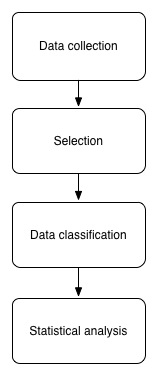
\includegraphics[scale=0.7]{gfx/methodology_diagram}\protect\caption{\label{fig:Research-methodology-diagram}Research methodology diagram}

\par\end{centering}

\selectlanguage{american}%
\selectlanguage{american}%
\end{figure}



\subsection{Data collection}

The data was obtained from an organization based in the Netherlands
that handles reports on online crime and fraud including phishing
in the form of phishing emails, which were reported between August
2013 and December 2013. The data consists of 8444 suspected phishing
emails in total that are selected and classified in the following
sections.


\subsection{\label{sub:Selection}Selection}

\begin{figure}[H]
\selectlanguage{american}%


\selectlanguage{english}%
\begin{centering}
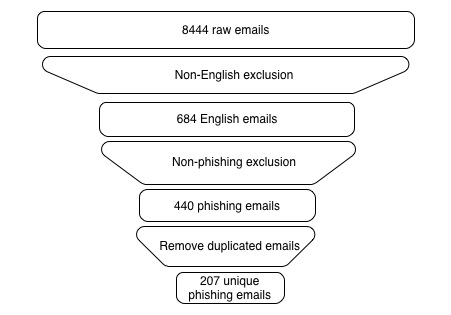
\includegraphics[scale=0.7]{gfx/selection}\protect\caption{\label{fig:Selection-diagram}Selection diagram}

\par\end{centering}

\selectlanguage{american}%
\selectlanguage{american}%
\end{figure}


The selection process consists of non-English exclusion, non-phishing
exclusion and removing duplicated emails. \autoref{fig:Selection-diagram}
illustrates the selection process.


\subsubsection{Non-English exclusion}

By manually inspecting each of suspected phishing emails, we can separate
the emails based on languages. These languages consist of English,
Dutch and other languages. The raw data was sorted by the subject
to help ease the separation process. This process gave the following
results:
\begin{itemize}
\item 7756 suspected phishing in Dutch language
\item 684 suspected phishing in English language
\item 4 suspected phishing in other languages
\end{itemize}
We excluded the suspected phishing emails in non-English languages
because our proficiency of non-English languages is not sufficient.
More detail on why we excluded the emails with non-English languages
can be found in \autoref{sec:Limitation} and \autoref{sec:Future-work}. 


\subsubsection{Non phishing exclusion}

From 684 suspected phishing emails in the English group, we excluded
the non-phishing emails by categorizing them into Phishing, Legitimate
and Others groups. The phishing group consists of the emails that
were indeed phishing. The legitimate group consists of legitimate
emails. The others group contains spam emails that represent commercial
advertisements and the emails that have no content -- for instance,
when the content has been removed before it was forwarded. 

This process gave the following results:
\begin{itemize}
\item 440 Phishing
\item 18 Legitimate
\item 226 Others 
\end{itemize}
Interestingly, based on the results of the categorization process,
we found 18 legitimate emails that were mistakenly reported as phishes
(i.e. false positives). This suggests that although there are only
18 false positives, misinterpretation of a fraudulent email among
the reporters is still occurred.


\subsubsection{Removing duplicated emails}

We coded the 440 phishing emails to an Excel sheet with necessary
variables so that we could convert the Excel sheet into an SPSS readable
file. Our aim was to analyze only the unique phishing emails, so that
the dataset would not be redundant. Duplicated emails in our dataset
were defined as those having exactly the same text in the entire body
of the emails. To find duplicated phishing emails, we conducted the
following steps:
\begin{enumerate}
\item Sorting the 440 emails by the subject, to show which emails had the
same subject.
\item Manually investigating each email with other emails with the same
subject to make sure all the text in the entire body is exactly the
same. If it did we excluded it.
\item Sometimes duplicated emails have slightly different subjects. To find
more duplicated emails, we searched based on random phrase from the
body.
\item If other emails found, we manually investigate each email to make
sure they had exactly the same text in the entire body.
\item We indicate the number of duplicated emails in ``CounterSameContents''
variable that we explain in \autoref{sub:variables}.
\end{enumerate}
These steps gave 207 unique phishing emails.


\subsection{Data Classification}

We classified our data into our variables to give a usable dataset
that could be analyzed. We put either 0 or 1 in our variables except
Mail ID, Timestamps, CountMessageReporter, Target and Reason variables.
For example, when a phishing email had a PDF attachment, we put value
\textquotedblleft 1\textquotedblright{} in our \textquotedblleft PDFattachment\textquotedblright{}
variable. Similarly, if the phishing email had a hyperlink in the
content, we put value \textquotedblleft 1\textquotedblright{} in our
\textquotedblleft ContainHyperlink\textquotedblright{} variable. As
we want to analyze our dataset based on Cialdini\textquoteright s
persuasion principles, it is important for us to explain our rationale
and conception based on Cialdini\textquoteright s principles. We explain
our variables and persuasion conception in the following sections.


\subsubsection{\label{sub:variables}Variables and concepts}

As we studied phishing email properties in \autoref{sub:Stop-phishing-at},
variables are needed to code our dataset into, so that we can conduct
the statistical analysis in the SPSS application. Based on our findings
in the literature survey on phishing email properties, 23 Variables
were created as part of the methodology processes prior to data classification.
Generic properties are depicted by the structural properties in phishing
emails except persuasion principles. The variables are explained in
the following list:
\begin{enumerate}
\item \emph{Mail ID} : Unique ID {[}Scale measurement{]}
\item \emph{Timestamps}: Implies the date and time when the email is reported
{[}Scale measurement{]}
\item \emph{Attachments:} Indicates whether the phishing email has an attachment(s),
and if so, what kind of attachment:

\begin{enumerate}
\item PDF {[}0 = No, 1 = Yes{]}
\item ZIP {[}0 = No, 1 = Yes{]}
\item HTML {[}0 = No, 1 = Yes{]}
\end{enumerate}
\item \textit{Instructions}: Implies the inquiry by the phishers in the
contents:

\begin{enumerate}
\item ReqOpenAttachment; A request to respond by opening an attachment(s)
{[}0 = No, 1 = Yes{]}
\item ReqClickLink; A request to respond by clicking URL(s) {[}0 = No, 1
= Yes{]}
\item ReqEmailReply; A request to respond by email reply {[}0 = No, 1 =
Yes{]}
\item ReqCallingByPhone; A request to respond by phone {[}0 = No, 1 = Yes{]}
\end{enumerate}
\item \emph{Contents}: Indicates what elements are included in the body

\begin{enumerate}
\item ContainHyperlink {[}0 = No, 1 = Yes{]}
\item UseHTML {[}0 = No, 1 = Yes{]}
\item IncludesImage {[}0 = No, 1 = Yes{]}
\end{enumerate}
\item \emph{HiddenURL}: Specifies whether a phishing email has a hidden
URL(s) {[}0 = No, 1 = Yes{]}
\item \emph{CountMessageReporter}: A counter where the reporter includes
extra information with the minimum value 0. For instance, when a reporter
said \textquotedblleft Geen spam, maar phishing!\textquotedblright{}
(\textquotedblleft Not spam, but phishing!\textquotedblright ), we
put a value 1 in this variable {[}Nominal measurement{]}
\item \emph{Target}: Determined the target institutions

\begin{enumerate}
\item TargetType {[}Values can be seen in \autoref{tab:Target-classification}{]}
\end{enumerate}
\item \emph{Reason}: Implies the reason why the unsuspected victim must
grant the phisher's request

\begin{enumerate}
\item ReasonType {[}Values can be seen in \autoref{tab:Reason-classification-1}{]}
\end{enumerate}
\item \emph{Cialdini's Principles}: Specifies what principle(s) the phishing
email signifies:

\begin{enumerate}
\item Reciprocation {[}0 = No, 1 = Yes{]}
\item Consistency {[}0 = No, 1 = Yes{]}
\item SocialProof {[}0 = No, 1 = Yes{]}
\item Likeability {[}0 = No, 1 = Yes{]}
\item Authority {[}0 = No, 1 = Yes{]}
\item Scarcity {[}0 = No, 1 = Yes{]}
\end{enumerate}
\item \emph{CounterSameContents}: A number that specifies how many emails
are duplicated. The minimum value of this variable is 1, which indicates
a unique email. For example, value 2 indicates that there is (2-1)
duplicated email with the same text in the body, value 3 means there
are (3-1) duplicated emails. The reason for this variable was to make
sure we can track back from 207 unique phishing emails to 440 phishing
emails.
\end{enumerate}
We established the variables based on the phishing email properties.
We also distinguished generic properties and persuasion properties.
The generic properties of a phishing email is affected by these variables:
attachments, requests, contents, hiddenURL, target and reason. On
the other hand, the persuasion properties are affected by these variables:
reciprocation, consistency, social proof, likeability, authority and
scarcity.


\subsubsection{\label{sub:cialdini}Cialdini's principles and conception}

As part of our analysis, we analyzed the phishing emails dataset based
on Cialdini\textquoteright s principles entitled \textquotedblleft The
science of persuasion\textquotedblright . The decision-making and
the rationale in this process are achieved based on our perspective
of Cialdini\textquoteright s principles in the following details. 

\textit{Reciprocation}: The norm that obligates individuals to repay
in kind what they have received. In other words, to return the favor,
or adjust to smaller request \cite{cialdini:2001}. This occurs when
a phisher sends an email containing a message that is perceived as
a request or obligation towards the recipient to \textquotedblleft return
the favor\textquotedblright . It might be natural for an individual
to feel \textquotedblleft obliged\textquotedblright{} to return the
favor for things or information that he/she is given and deems to
be valuable. For example, in the phishing email context, when PayPal
has detected there are suspicious activities on our account, we sometimes
believe that PayPal has done a good job in detecting security risk
on their system and we feel \textquotedblleft obliged\textquotedblright{}
to return the favor of that valuable information. Another example
is that if the sender gave the information that they have added \textquotedblleft extra
security\textquotedblright{} on their system we also feel obliged
to grant their request.

\emph{Consistency}: Public commitment occurs when people become psychologically
become vested in a decision they have made \cite{workman:2008}. This
happens when a phishing email contains a message that is perceived
to request the recipient's \textquotedblleft consistency\textquotedblright{}
on a decision they have made. For example in the phishing email context,
when a hotel agent asks us to review the payment details of our reservation
that we have previously made, we might feel committed or agreed to
review the payment details that have been given. Another example is
if \textquotedblleft Facebook\textquotedblright{} gives a link to
change your password when you previously requested to change it. It
might be not applicable to those who are not requesting password previously,
but we believe it will impact on those who previously committed to
change their password. 

\emph{Social proof}: This occurs when people model the behavior of
their peer group, role models, important others or because it is generally
\textquotedbl{}fashionable\textquotedbl{} \cite{workman:2008}. For
example, when someone tells us that there are hundreds of other people
who use a particular system, we might want to agree to use it as well
just because a lot of other people use it. Another example is when
Facebook gives information that someone wants to be our friend, and
we know who that someone is. We might tend to follow that request
and click the link to accept the request. 

\emph{Likeability}: It occurs when people trust and comply with requests
from others who they find attractive or are perceived as credible
and having special expertise or abilities such as sports figures or
actors they like \cite{workman:2008}. In the context of a phishing
email, the email contains a message that attracts the recipient to
comply with the sender's request, based on reference on something
or someone likeable for the recipient. Cialdini \cite{cialdini:2001}
identified that people usually \textquotedblleft trust those they
like\textquotedblright . For example, if someone is asking us to download
and listen to music that Michael Jackson made, we might be attracted
to download and listen to it just because we happen to love Michael
Jackson's music. It is like someone asks us to watch a concert and
they said, \textquotedblleft Coldplay will be there\textquotedblright .
If we are a devoted fan of Coldplay, we might find it very interesting.
Another example is when a sender gives compliments to us or commits
to help us safeguard our account from hackers, we tend to think that
the sender cares about our safety, which is good for us, and consequently
it might attract us to comply with the sender's request. 

\emph{Authority}: It can be used to engender fear, where people obey
commands to avoid negative consequences such as losing a privilege
or something of value, punishment, humiliation or condemnation \cite{workman:2008}.
This happens when a phishing email contains a logo, image, signature
or anything that looks like a legitimate institution. It can be used
to makes it look trustworthy so that the recipient might accept and
obey the sender's request. For example, an email may present a somewhat
authentic-looking signature like \textquotedblleft Copyright 2013
PayPal, Inc. All rights reserved\textquotedblright{} or with the PayPal
logo. Cialdini \cite{cialdini:2001} suggests that authoritative persuasion
can be achieved by presenting an \textquotedblleft aura of legitimacy\textquotedblright .
Another example is when the content of the email states that it is
from the \textquotedblleft System Administrator\textquotedblright{}
asking for password update. It would be not authoritative if random
people asked us to change our password.

\emph{Scarcity}: This is based on the principle of reactance, where
people respond to perceived shortages by placing greater psychological
value on perceived scarce items \cite{workman:2008}. A phishing email
containing such a message tells a recipient to react or respond to
scarce/becoming-scarce items, things or privileges. In the phishing
email context, if a sender tells us that he/she will suspend/deactivate/limit
our account if we do not respond to his/her request, we might want
to respond to their request because we are worried we will not able
to access our account again -- in other words, our account becomes
scarce or limited.

\begin{figure}[H]
\begin{centering}
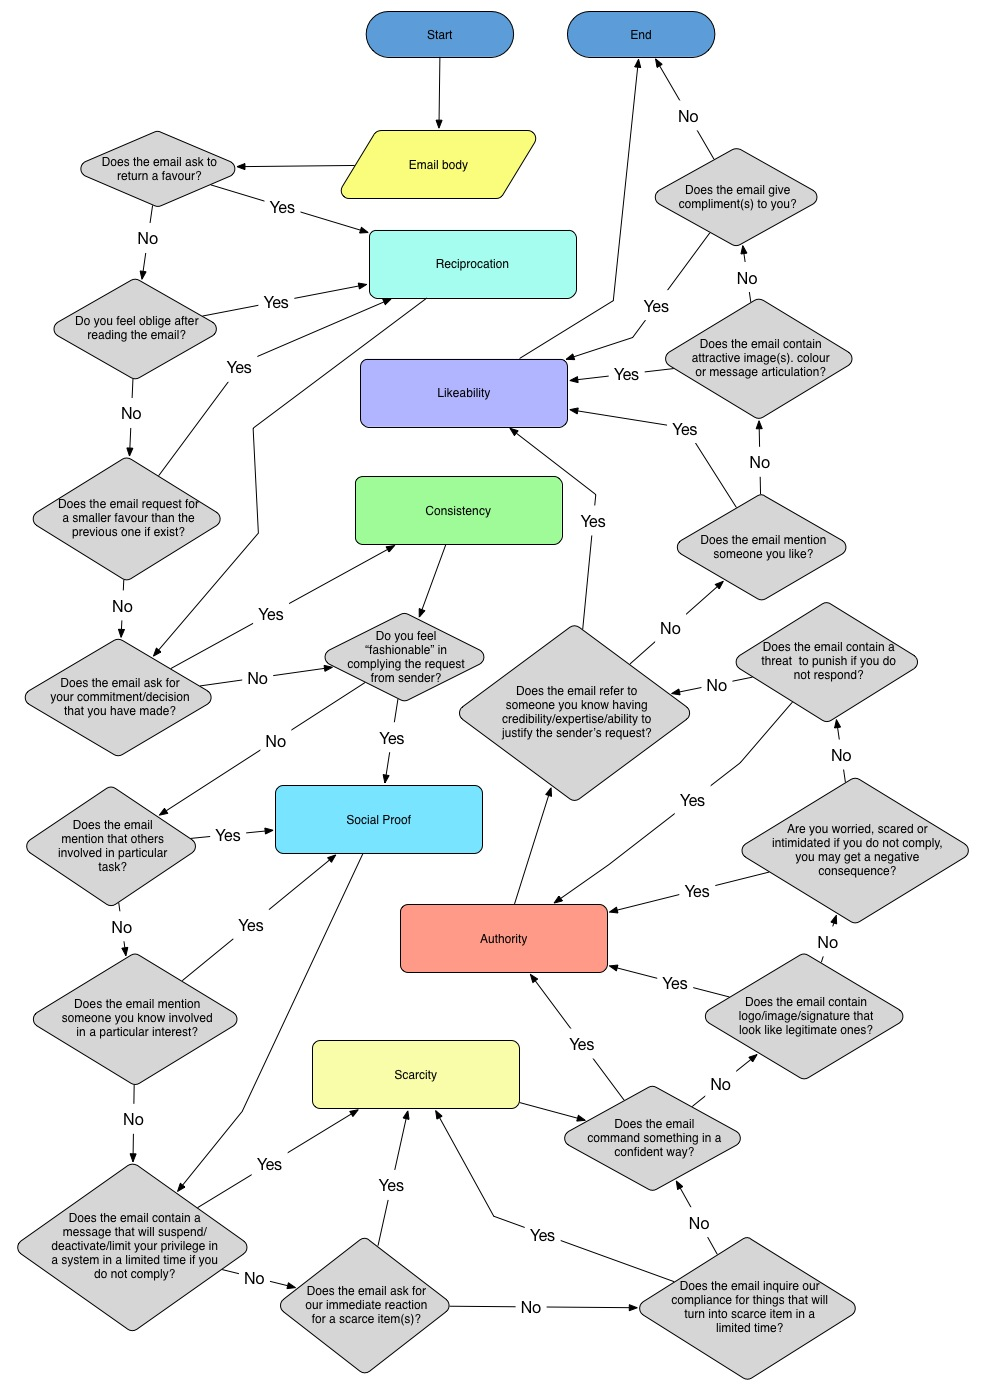
\includegraphics[scale=0.4]{gfx/pseudo-cialdini-2}
\par\end{centering}

\protect\caption{\label{fig:Flowchart-cialdini}Integration pseudo-code of Cialdini's
principles}
\end{figure}


We have made a flowchart%
\footnote{Shapes and lines were created based on http://www.rff.com/how\_to\_draw\_a\_flowchart.htm%
} in \autoref{fig:Flowchart-cialdini} that illustrates our analysis
of the dataset based on Cialdini's principles. 


\subsection{Statistical analysis}

In the previous section, we described the framework of our methodology
in considerable detail. Until data classification, we used Microsoft
Excel to code our data. To perform the analyses, we transformed the
data into an SPSS readable file. We initially recorded our data in
23 variables that could be expanded depending on our analyses, such
as selecting cases that have all instructions or selecting a specific
target sector.

The data was analyzed by quantitative analysis from three different
viewpoints: general properties characteristics, persuasion principles
characteristics, and their relationships. We used frequency analysis
to answer questions related to occurrences. For instance, we used
frequency analysis to answer the most targeted institution in \autoref{chap:research-questions}.
Furthermore, we used Pearson chi-square to test our hypotheses to
discover if there was a significant relationship between two variables.
If the resulted p-value was less than 0.05, 0.01, or 0.001, we are
95\%, 99\% and 99.9\% confident, respectively, that the two chosen
variables have a significant relationship. By combining frequency
analysis and chi-square test, we see how they can answer our research
questions in the next section. 

As our data is not continuous (i.e. interval or ratio) but nominal
(i.e. categorical), we do not analyze our data by Pearson correlation.
However, to test the strength of association involving nominal variables,
the appropriate measurements are using phi and Cramer\textquoteright s
V. Phi is used for 2 by 2 tables and Cramer\textquoteright s V can
be used for more than 2 by 2 tables. Since our data is analyzed on
a 2 by 2 table, Phi measurements are used. Values close to 0 indicate
a very weak relationship, and values close to -1 or +1 indicate a
very strong negative or positive relationship respectively.


\section{Results}

In this section, we elaborate on the results we obtained through our
analyses. We begin this section by describing the frequency analyses
of the general structural properties and persuasion principles. We
then describe the relationship analysis between the general structural
properties and the persuasion principles. We conclude the section
by mentioning the results related to persuasion principles used in
phishing emails.

We find that 36.2\% of the total phishing emails have attachment(s)
included within their content. 63.8\% of them therefore do not have
attachments. Of the emails with attachments, 4\% have PDF attachments,
78.7\% have ZIP attachments, 12\% have HTML attachments and 5.3\%
of them have had the attachments removed before the emails were forwarded. 

We are not sure what type of attachments they had, but we determined
that an attachment element was there if there was a request to open
an attachment within the email content. For example, in an email dated
December 20th 2013 11:29am, it was said in the email's body: \textquotedblleft ...we
have sent the attached as a secure electronic file\textquotedblright .
As nothing was actually attached, we suspect it was removed by antivirus
software. \autoref{tab:Attachment(s)-analysis} illustrates our findings
on attachment variables. 

When we look deeper, we find that there is a significant relationship
between ZIP file and Attachment variable. A chi-square test resulted
in $X^{2}(1)=145.236,p<0.001$. Similarly, there is a significant
association between HTML file and Attachment variable with a chi-square
test resulting in $X^{2}(1)=16.560,p<0.001$. However when we test
the relationship between PDF and attachment, the significance level
is not as strong as ZIP and HTML, with $X^{2}(1)=5.358,p=0.021$.

\begin{table}[H]
\begin{centering}
\begin{tabular}{ccc}
\toprule 
Type of attachment & \textsc{Frequency} & \textsc{Percent}\tabularnewline
\midrule
\midrule 
{\footnotesize{}ZIP } & {\footnotesize{}59} & {\footnotesize{}78.7}\tabularnewline
\midrule 
{\footnotesize{}HTML } & {\footnotesize{}9} & {\footnotesize{}12}\tabularnewline
\midrule 
{\footnotesize{}Removed } & {\footnotesize{}4} & {\footnotesize{}5.3}\tabularnewline
\midrule 
{\footnotesize{}PDF} & {\footnotesize{}3} & {\footnotesize{}4}\tabularnewline
\midrule 
\textsc{\footnotesize{}Total} & {\footnotesize{}75} & {\footnotesize{}100}\tabularnewline
\bottomrule
\end{tabular}\protect\caption{\label{tab:Attachment(s)-analysis}Attachment analysis}

\par\end{centering}

\selectlanguage{american}%
\selectlanguage{american}%
\end{table}


\ 

When we look at the instructions or requests used in the dataset,
we find 202 emails or (97.6\% of total) with clear instructions: requests
to click URL(s); requests to open attachments; requests to reply by
email; or requests to respond by phone. 2.4\% of the total emails
do not contain a clear instructions to the recipients. For instance,
on 24 November 2013 at 19:59, an email was sent that only include
an attachment but no instruction to open it. However, with the subject
of \textquotedblleft Payrolls reports\textquotedblright{} we have
the impression that this is a targeted phishing email, which means
it only aims at a small audience as the recipients, usually a certain
institution. Similarly, an email sent 15 August 2013 at 17:38 contains
HTML suggesting a recipient to check the interesting pages on Facebook.
However, there are no instructions to click on the URL, nor any other
instructions. 

Apart from the instruction to click URL(s), we find that 37.2\% of
the total phishing emails request to open attachments, 52.7\% of them
request to click URLs, 16.9\% request for email replies and 4.3\%
request a phone call. Moreover, one single email can contain multiple
requests. If we look deeper, we have 8 valid emails (3.9\% of all
emails) that have requests to both open attachments and click URLs.
However, we do not find any email which has all requests in the content.

\autoref{tab:Methods-analysis} illustrates our findings in respect
of requests used. Of all phishing emails that have clear instructions,
54\% request to click URL(s), 38.1\% request to open attachment(s),
17.3\% request an email reply and 4.5\% request a response by calling
on the phone.

\begin{table}[H]
\begin{centering}
\begin{tabular}{ccc}
\toprule 
\textsc{\small{}Request} & \textsc{\small{}Frequency} & \textsc{\small{}Percent}\tabularnewline
\midrule
\midrule 
{\small{}click URL} & {\small{}109} & {\small{}52.7}\tabularnewline
\midrule 
{\small{}open Attachment(s)} & {\small{}77} & {\small{}37.2}\tabularnewline
\midrule 
{\small{}Email Reply} & {\small{}35} & 16.9\tabularnewline
\midrule 
{\small{}call by phone} & {\small{}9} & {\small{}4.3}\tabularnewline
\bottomrule
\end{tabular}\protect\caption{\label{tab:Methods-analysis}Request analysis of all total emails
(one email can contain more than one instructions so the total here
does not sum up to 100\%)}

\par\end{centering}

\selectlanguage{american}%
\selectlanguage{american}%
\end{table}


\ 

As we discussed before, we have analyzed the content of phishing emails
in our corpus. We looked at whether they had URLs, use HTML code or
included images within its content. We find that 60.4\% have URLs,
while 39.6\% do not. 66.2\% of the emails use HTML code while 33.8\%
do not use. Finally, 35.3\% of them include images while 64.7\% do
not. \autoref{tab:Content-analysis} highlights our findings in respect
of content analysis. The percentage depicted is of all total emails.
If we look further at all emails that utilized HTML, 120 emails (87.6\%)
provided URLs, and 73 (53.3\%) include images. Furthermore, of all
73 emails that include images, 67 emails (91.8\%) provided URLs. Based
on these result, we know that one variable overlap with other variables.
Therefore, the total percentage does not sum up to 100\%.

\begin{table}[h]
\centering{}%
\begin{tabular}{ccc}
\toprule 
\textsc{\small{}Content} & \textsc{\small{}Frequency} & \textsc{\small{}Percent}\tabularnewline
\midrule
\midrule 
{\small{}utilizing HTML} & {\small{}137} & 66.2\tabularnewline
\midrule 
{\small{}URL presence} & {\small{}125} & 60.4\tabularnewline
\midrule 
{\small{}include Image} & {\small{}73} & {\small{}35.3}\tabularnewline
\bottomrule
\end{tabular}\protect\caption{\label{tab:Content-analysis}Content analysis of all total emails
(one email can contain more than one content variables so the total
here does not sum up to 100\%)}
\end{table}


\ 

When we look at the target classification table in \autoref{tab:Target-analysis},
we find that financial sector is the most targeted sector and ISP
is the least common target in our corpus. Furthermore, e-Commerce/retail
sector, administrator and government are the second, third and fourth
most targeted sectors, respectively. When we look deeper at the detailed
list of targeted brands, we find PayPal has the highest frequency
(37.2\%) of the total financial targeted emails. Bank of America contributes
6.4\%, American Express 5.1\%, Visa contributes 5.1\% and Western
Union contributes 3.8\%. Other financial institutions contribute to
less than 3\%. \autoref{fig:Detailed-of-financial} illustrates the
detailed target brands of the financial sector.

As one email does not have more than 1 targeted sector, the total
sums up to 100\%. Note that we initially had 92 targets in our corpus
and we had to classify them into 10 target types in our data classification.

\begin{table}[h]
\begin{centering}
\begin{tabular}{ccc}
\toprule 
\textsc{\small{}Target} & \textsc{\small{}Frequency} & \textsc{\small{}Percent}\tabularnewline
\midrule
\midrule 
{\small{}Financial} & {\small{}78} & {\small{}37.7}\tabularnewline
\midrule 
{\small{}E-commerce/retails} & {\small{}40} & {\small{}19.3}\tabularnewline
\midrule 
{\small{}Administrator} & {\small{}30} & {\small{}14.5}\tabularnewline
\midrule 
{\small{}Government} & {\small{}14} & {\small{}6.8}\tabularnewline
\midrule 
{\small{}Non-existence/individual} & {\small{}13} & {\small{}6.3}\tabularnewline
\midrule 
{\small{}Social media} & {\small{}11} & {\small{}5.3}\tabularnewline
\midrule 
{\small{}Postal service} & {\small{}9} & {\small{}4.3}\tabularnewline
\midrule 
{\small{}Travel agency} & {\small{}5} & {\small{}2.4}\tabularnewline
\midrule 
{\small{}Industrial} & {\small{}5} & {\small{}2.4}\tabularnewline
\midrule 
{\small{}ISP} & {\small{}2} & {\small{}1}\tabularnewline
\midrule
\midrule 
\textsc{\small{}Total} & \textsc{\small{}207} & \textsc{\small{}100}\tabularnewline
\bottomrule
\end{tabular}
\par\end{centering}

\begin{centering}
\protect\caption{\label{tab:Target-analysis}Target analysis}

\par\end{centering}

\selectlanguage{american}%
\selectlanguage{american}%
\end{table}


When we look at what reasons are used in \autoref{tab:Reason-classification},
we find that 48.8\% of the total emails are account related, 25\%
have a financial reason and 11.1\% a document-related reason. Only
9.7\% have a product/services reason and only 4.8\% a social reason.
When we break these down, account-related reasons consists of a security
risk that contributes 28.7\%, and system upgrade, new system requirement
and account expiration that contribute below 11\%. This suggests that
an account-related reason is the most common pretext to manipulate
recipients in our corpus while social is evidently the least common
pretext. \autoref{fig:Detailed-account-related} illustrates the detailed
list of account-related reasons.

\begin{table}[h]
\centering{}%
\begin{tabular}{ccc}
\toprule 
\textsc{\small{}Reason} & \textsc{\small{}Frequency} & \textsc{\small{}Percent}\tabularnewline
\midrule
\midrule 
{\small{}Account related} & {\small{}101} & 48.8\tabularnewline
\midrule 
{\small{}Financial incentive} & {\small{}53} & 25.6\tabularnewline
\midrule 
{\small{}Document related} & {\small{}23} & {\small{}11.1}\tabularnewline
\midrule 
Product/services & 20 & 9.7\tabularnewline
\midrule 
Social  & 10 & 4.8\tabularnewline
\midrule
\midrule 
\textsc{\small{}Total} & 207 & 100\tabularnewline
\bottomrule
\end{tabular}\protect\caption{\label{tab:Reason-classification}Reason classification}
\end{table}


\begin{figure}[h]
\selectlanguage{american}%


\selectlanguage{english}%
\begin{centering}
\includegraphics[scale=0.6]{\string"gfx/reasons_detailed_17september2014_bar chart1\string".jpg}\protect\caption{\label{fig:Detailed-account-related}Detailed account related reason
graph}

\par\end{centering}

\selectlanguage{american}%
\selectlanguage{american}%
\end{figure}


We look at the result of persuasion techniques analysis based on Cialdini's
principles with our corpus. As we can see from \autoref{tab:Persuasion-principle-analysis},
we find that 96.1\% of the total phishing emails are using authority
principle, which is the most used technique in our dataset, followed
by the scarcity principle at 41.1\%. 21.7\% of the total use the likeability
principle, while 17.4\% use the consistency principle. 9.7\% use the
reciprocation principle and 5.3\% of them use the social proof principle.
Since the authority principle is the highest persuasion technique
in our corpus, it is interesting to know why phishers often use authority
as the main technique. Perhaps, most people do not want negative consequences
as a result of disobedience to authoritative figures. Consequently,
those people who respond more obediently to authority are more likely
to comply with the emails\textquoteright{} requests than people who
are more skeptical about authoritative figures. Note that one email
can use multiple principles. Therefore, the total percentage does
not sum up to 100\%.

\begin{table}[h]
\centering{}%
\begin{tabular}{ccc}
\toprule 
\textsc{\small{}Cialdini's principles} & \textsc{\small{}Frequency} & \textsc{\small{}Percent}\tabularnewline
\midrule
\midrule 
{\small{}Authority} & 199 & 96.1\tabularnewline
\midrule 
{\small{}Scarcity} & 85 & 41.1\tabularnewline
\midrule 
{\small{}Likeability} & 45 & 21.7\tabularnewline
\midrule 
Consistency & 36 & 17.4\tabularnewline
\midrule 
Reciprocation & 20 & 9.7\tabularnewline
\midrule 
Social proof & 11 & 5.3\tabularnewline
\bottomrule
\end{tabular}\protect\caption{\label{tab:Persuasion-principle-analysis}Persuasion principles analysis}
\end{table}


Based on the results of persuasion principles analysis, we know that
the authority principle is the most used principle in our corpus.
Now, we look at the relationship between government and authority
principle to test hypothesis 1. We find that 95.9\% of non-government
targeted emails use the authority principle, while 4.1\% of them do
not impersonate government nor use the authority principle. We find
100\% of government-targeted emails have the authority principle.
On the other hand, we find 93\% of all authority emails are non-government
targeted emails and 7\% of them are government-targeted emails. \autoref{tab:Government-and-authority}
depicts the relationship between government-targeted emails and the
authority principle. Furthermore, of all phishing emails, 6.8\% of
them both use the authority principle and target the government sector.
A chi-square test was performed and we find that there is no significant
association between the government sector and authority principle,
as $X^{2}(1)=0.604,p=0.473$. Since p is not less than 0.05, we reject
hypothesis 1.

\begin{minipage}[t]{1\columnwidth}%
\begin{longtable}{cccc}
\caption{\label{tab:Government-and-authority}Government sector and authority
principle}
\tabularnewline
\toprule 
\textsc{\footnotesize{}Type of Target} & {\footnotesize{}Non-authority} & {\footnotesize{}Authority} & \multirow{1}{*}{{\footnotesize{}N}}\tabularnewline
\midrule 
\multirow{1}{*}{{\footnotesize{}Non-government}} & {\footnotesize{}8} & {\footnotesize{}185} & \multirow{1}{*}{{\footnotesize{}193}}\tabularnewline
\midrule 
\multirow{1}{*}{{\footnotesize{}Government}} & {\footnotesize{}0} & {\footnotesize{}14} & \multirow{1}{*}{{\footnotesize{}14}}\tabularnewline
\midrule
\midrule 
{\footnotesize{}N} & {\footnotesize{}8} & {\footnotesize{}199} & {\footnotesize{}207}\tabularnewline
\midrule
\midrule 
{\footnotesize{}Pearson chi-square} & \multicolumn{3}{c}{{\footnotesize{}0.604}}\tabularnewline
\midrule
\end{longtable}%
\end{minipage}

When we look at the relationship between phishing emails that impersonate
administrators and the authority principle to test hypothesis 2, we
find that 96.7\% of administrator-targeted emails use the authority
principle and 96\% of non-administrator emails use the authority principle.
On the other hand, 85.4\% of all authority emails are non-administrator
and 14.6\% of them are administrator-targeted emails. A chi-square
test was performed and we find that there is no significant relationship
between administrator target and authority principle, $X^{2}(1)=0.027,p=0.870$.
Since p is not less than 0.05, we reject hypothesis 2. \autoref{tab:Administrator-sector-and}
highlights the relationship between administrator sector and the authority
principle.

\begin{minipage}[t]{1\columnwidth}%
\begin{longtable}{cccc}
\caption{\label{tab:Administrator-sector-and}Administrator sector and authority
principle }
\tabularnewline
\toprule 
\textsc{\footnotesize{}Type of Target} & {\footnotesize{}Non-authority} & {\footnotesize{}Authority} & \multirow{1}{*}{{\footnotesize{}N}}\tabularnewline
\midrule 
\multirow{1}{*}{{\footnotesize{}Non-administrator}} & {\footnotesize{}7} & {\footnotesize{}170} & \multirow{1}{*}{{\footnotesize{}177}}\tabularnewline
\midrule 
\multirow{1}{*}{{\footnotesize{}Administrator}} & {\footnotesize{}1} & {\footnotesize{}29} & \multirow{1}{*}{{\footnotesize{}30}}\tabularnewline
\midrule
\midrule 
{\footnotesize{}N} & {\footnotesize{}8} & {\footnotesize{}199} & {\footnotesize{}207}\tabularnewline
\midrule
\midrule 
{\footnotesize{}Pearson chi-square} & \multicolumn{3}{c}{{\footnotesize{}0.027}}\tabularnewline
\midrule
\end{longtable}%
\end{minipage}

Now we look at the association between financial sector and scarcity
principle to test hypothesis 3. We find that 39.7\% of all phishing
emails that target financial sector use the scarcity principle, while
60.3\% do not. Furthermore, 41.9\% of all non-financial targeted emails
use the scarcity principle, while 58.1\% do not. 63.5\% of scarcity
emails are non-financial targeted emails, while 36.5\% of them are
financial targeted emails. We performed a chi-square test and we found
that there is no significant association between the financial sector
and scarcity principle, with $X^{2}(1)=0.090,p=0.764$. Since p is
not less than 0.05, we reject hypothesis 3. \autoref{tab:Financial-sector-and}
illustrates the relationship between financial-targeted emails and
the scarcity principle.

\begin{minipage}[t]{1\columnwidth}%
\begin{longtable}{cccc}
\caption{\label{tab:Financial-sector-and}Financial sector and scarcity principle}
\tabularnewline
\toprule 
{\footnotesize{}Type of Target} & {\footnotesize{}Non-scarcity} & {\footnotesize{}Scarcity} & \multirow{1}{*}{{\footnotesize{}N}}\tabularnewline
\midrule 
\multirow{1}{*}{{\footnotesize{}Non-financial}} & {\footnotesize{}75} & {\footnotesize{}54} & \multirow{1}{*}{{\footnotesize{}129}}\tabularnewline
\midrule 
\multirow{1}{*}{{\footnotesize{}Financial}} & {\footnotesize{}47} & {\footnotesize{}31} & \multirow{1}{*}{{\footnotesize{}78}}\tabularnewline
\midrule
\midrule 
{\footnotesize{}N} & {\footnotesize{}122} & {\footnotesize{}85} & {\footnotesize{}207}\tabularnewline
\midrule
\midrule 
{\footnotesize{}Pearson chi-square} & \multicolumn{3}{c}{{\footnotesize{}0.090}}\tabularnewline
\midrule
\end{longtable}%
\end{minipage}

Turning our attention to the association between phishing emails that
target the e-commerce/retail sector and the likeability principle,
we can test hypothesis 4. We find that 20\% of e-commerce/retail sector
targeted emails use the likeability principle. Furthermore, 22.2\%
of non e-commerce/retail sector targeted emails use the likeability
principle. On the other hand, only 17.8\% of all likeability emails
are e-commerce/retail sector targeted emails. A chi-square test was
performed and we found that there is no significant association between
phishing emails targeting the e-commerce/retail sector and the likeability
principle, with $X^{2}(1)=0.088,p=0.767$. Since p is not less than
0.05, we reject hypothesis 4. \autoref{tab:E-commerce/retails-sector-and}
illustrates the relationship between the e-commerce/retail targeted
sector and the likeability principle.

\begin{minipage}[t]{1\columnwidth}%
\begin{longtable}{cccc}
\caption{\label{tab:E-commerce/retails-sector-and}E-commerce/retails sector
and likeability principle}
\tabularnewline
\toprule 
{\footnotesize{}Type of Target} & {\footnotesize{}Non-likeability} & {\footnotesize{}Likeabillity} & \multirow{1}{*}{{\footnotesize{}N}}\tabularnewline
\midrule 
\multirow{1}{*}{{\footnotesize{}Non-ecomm/retails}} & {\footnotesize{}130} & {\footnotesize{}37} & \multirow{1}{*}{{\footnotesize{}167}}\tabularnewline
\midrule 
\multirow{1}{*}{{\footnotesize{}Ecomm/retails}} & {\footnotesize{}32} & {\footnotesize{}8} & \multirow{1}{*}{{\footnotesize{}40}}\tabularnewline
\midrule
\midrule 
{\footnotesize{}N} & {\footnotesize{}162} & {\footnotesize{}45} & {\footnotesize{}207}\tabularnewline
\midrule
\midrule 
{\footnotesize{}Pearson chi-square} & \multicolumn{3}{c}{{\footnotesize{}0.088}}\tabularnewline
\midrule
\end{longtable}%
\end{minipage}

Now we look at the association between phishing emails targeting social
media and the social proof principle to test hypothesis 5. We find
that 18.2\% of social media targeted emails employ the social proof
principle. Furthermore, 4.6\% of non-social media targeted emails
employ the social proof principle. 18.2\% of all social proof emails
are social media targeted emails and 81.8\% of them are not. A chi-square
test was performed and we found that there is no significant association
between phishing emails targeting social networks and social proof
principle, with $X^{2}(1)=3.823,p=0.051$. Therefore since p is not
less than 0.05, we reject hypothesis 5. \autoref{tab:Social-media-sector}
depicts the relationship between social media and the social proof
principle.

\begin{minipage}[t]{1\columnwidth}%
\begin{longtable}{cccc}
\caption{\label{tab:Social-media-sector}Social media sector and social proof}
\tabularnewline
\toprule 
{\footnotesize{}Type of Target} & {\footnotesize{}Non-social proof} & {\footnotesize{}social proof} & \multirow{1}{*}{{\footnotesize{}N}}\tabularnewline
\midrule 
\multirow{1}{*}{{\footnotesize{}Non-social media}} & {\footnotesize{}187} & {\footnotesize{}9} & \multirow{1}{*}{{\footnotesize{}196}}\tabularnewline
\midrule 
\multirow{1}{*}{{\footnotesize{}Social media}} & {\footnotesize{}9} & {\footnotesize{}2} & \multirow{1}{*}{{\footnotesize{}11}}\tabularnewline
\midrule
\midrule 
{\footnotesize{}N} & {\footnotesize{}196} & {\footnotesize{}11} & {\footnotesize{}207}\tabularnewline
\midrule
\midrule 
{\footnotesize{}Pearson chi-square} & \multicolumn{3}{c}{{\footnotesize{}3.823}}\tabularnewline
\midrule
\end{longtable}%
\end{minipage}

Next, we look at the relationship between authority principle and
scarcity principle to test hypothesis 6. Based on the result in \autoref{tab:Authority-and-scarcity},
we find that 41.7\% of authoritative emails use the scarcity principle
while 58.3\% do not. However, we find that 97.6\% of all scarcity
emails use the authority principle and only 2.4\% of them do not.
A chi-square test suggests that there is no significant relationship
between the authority principle and the scarcity principle, with $X^{2}(1)=0.887,p=0.346$.
Thus, we reject hypothesis 6.

\begin{minipage}[t]{1\columnwidth}%
\begin{longtable}{cccc}
\caption{\label{tab:Authority-and-scarcity}Authority and scarcity}
\tabularnewline
\toprule 
\selectlanguage{american}%
\selectlanguage{american}%
 & {\footnotesize{}Non-scarcity} & {\footnotesize{}Scarcity} & \multirow{1}{*}{{\footnotesize{}N}}\tabularnewline
\midrule 
\multirow{1}{*}{{\footnotesize{}Non-authority}} & {\footnotesize{}6} & {\footnotesize{}2} & \multirow{1}{*}{{\footnotesize{}8}}\tabularnewline
\midrule 
\multirow{1}{*}{{\footnotesize{}Authority}} & {\footnotesize{}116} & {\footnotesize{}83} & \multirow{1}{*}{{\footnotesize{}199}}\tabularnewline
\midrule
\midrule 
{\footnotesize{}N} & {\footnotesize{}122} & {\footnotesize{}85} & {\footnotesize{}207}\tabularnewline
\midrule
\midrule 
{\footnotesize{}Pearson chi-square} & \multicolumn{3}{c}{{\footnotesize{}0.887}}\tabularnewline
\midrule
\end{longtable}%
\end{minipage}

We now consider the relationship between the likeability principle
and the consistency principle to test hypothesis 7. Based on our results
in \autoref{tab:Likeability-and-consistency}, we find that only 6.7\%
of likeability emails have the consistency principle while 93.3\%
of them do not. In addition, we find that 20.4\% of non-likeability
emails have the consistency principle while 79.6\% of them do not.
On the other hand, 8.3\% of all consistency emails are likeability
emails while 24.6\% of non-consistency emails are likeability emails.
A chi-square test suggests that there is a significant relationship
between the likeability principle and the consistency principle, with
$X^{2}(1)=4.603,p=0.032$. Phi measurement suggests a very weak negative
(inverse) relationship at -0.149, indicating that as one variable
increases, the other variable decreases. This suggests that the higher
the use of the likeability principle in a phishing email, the less
chance of the consistency principle being used. Thus we accept hypothesis
7 that says the occurrence of the likeability principle will impact
the occurrence of consistency.

\begin{minipage}[t]{1\columnwidth}%
\begin{longtable}{cccc}
\caption{\label{tab:Likeability-and-consistency}Likeability and consistency}
\tabularnewline
\toprule 
\selectlanguage{american}%
\selectlanguage{american}%
 & {\footnotesize{}Non-consistency} & {\footnotesize{}Consistency} & \multirow{1}{*}{{\footnotesize{}N}}\tabularnewline
\midrule 
\multirow{1}{*}{{\footnotesize{}Non-likeability}} & {\footnotesize{}129} & {\footnotesize{}33} & \multirow{1}{*}{{\footnotesize{}162}}\tabularnewline
\midrule 
\multirow{1}{*}{{\footnotesize{}Likeability}} & {\footnotesize{}42} & {\footnotesize{}3} & \multirow{1}{*}{{\footnotesize{}45}}\tabularnewline
\midrule
\midrule 
{\footnotesize{}N} & {\footnotesize{}171} & {\footnotesize{}36} & {\footnotesize{}207}\tabularnewline
\midrule
\midrule 
{\footnotesize{}Pearson chi-square} & \multicolumn{3}{c}{{\footnotesize{}4.603{*}}}\tabularnewline
\midrule
\end{longtable}%
\end{minipage}

{*}p < 0.05 (significant).

\ 

Now we move on to find out the association between URL presence and
hidden URLs in our corpus to test hypothesis 8. Based on our results
in \autoref{tab:URL-presence-and}, we find that 76\% of URLs are
hidden while 24\% are not. A chi-square test suggests that there is
a highly significant association between URL presence and hidden URLs,
with $X^{2}(1)=115.191,p<0.001$. Moreover, Phi measurement suggests
a strong positive relationship at 0.746. This indicates a strong relationship
between them, so we accept hypothesis 8.

\begin{minipage}[t]{1\columnwidth}%
\begin{longtable}{cccc}
\caption{\label{tab:URL-presence-and}URL presence and obfuscated URL}
\tabularnewline
\toprule 
{\footnotesize{}URL} & {\footnotesize{}Not hidden} & {\footnotesize{}hidden} & \multirow{1}{*}{{\footnotesize{}N}}\tabularnewline
\midrule 
\multirow{1}{*}{{\footnotesize{}Not exist}} & {\footnotesize{}82} & {\footnotesize{}0} & \multirow{1}{*}{{\footnotesize{}82}}\tabularnewline
\midrule 
\multirow{1}{*}{{\footnotesize{}Exist}} & {\footnotesize{}30} & {\footnotesize{}95} & \multirow{1}{*}{{\footnotesize{}125}}\tabularnewline
\midrule
\midrule 
{\footnotesize{}N} & {\footnotesize{}112} & {\footnotesize{}95} & {\footnotesize{}207}\tabularnewline
\midrule
\midrule 
{\footnotesize{}Pearson chi-square} & \multicolumn{3}{c}{{\footnotesize{}115.191{*}{*}{*}}}\tabularnewline
\midrule
\end{longtable}%
\end{minipage}

{*}{*}{*} p < 0.001 (significant).

\ 

We now look at the relationship between URL presence and the emails
which request to click on URLs in \autoref{tab:URL-presence-and-1}
to test hypothesis 9. We find 87.2\% of phishing emails that have
URLs also requested receivers to click on them, while 12.8\% did.
A chi-square test was performed and suggests that there is a highly
significant relationship between URL presence and request to click
on URLs, $X^{2}(1)=151.034,p<0.001$. Phi measurement suggests that
they have a strong positive relationship at 0.854. Thus, this data
supports hypothesis 9.

\begin{minipage}[t]{1\columnwidth}%
\begin{longtable}{cccc}
\caption{\label{tab:URL-presence-and-1}URL presence and Request to click URL}
\tabularnewline
\toprule 
{\footnotesize{}URL} & {\footnotesize{}does not request to click URL} & {\footnotesize{}requests to click URL} & \multirow{1}{*}{{\footnotesize{}N}}\tabularnewline
\midrule 
\multirow{1}{*}{{\footnotesize{}Not exist}} & {\footnotesize{}82} & {\footnotesize{}0} & \multirow{1}{*}{{\footnotesize{}82}}\tabularnewline
\midrule 
\multirow{1}{*}{{\footnotesize{}Exist}} & {\footnotesize{}16} & {\footnotesize{}109} & \multirow{1}{*}{{\footnotesize{}125}}\tabularnewline
\midrule
\midrule 
{\footnotesize{}N} & {\footnotesize{}98} & {\footnotesize{}109} & {\footnotesize{}207}\tabularnewline
\midrule
\midrule 
{\footnotesize{}Pearson chi-square} & \multicolumn{3}{c}{{\footnotesize{}151.034{*}{*}{*}}}\tabularnewline
\midrule
\end{longtable}%
\end{minipage}

{*}{*}{*} p < 0.001 (significant).

\ 

Similarly, we look at the association between the emails that include
attachments and the emails which request to open attachments to test
hypothesis 10. Based on our results in \autoref{tab:Includes-attachment-and},
96\% of phishing emails that include attachments also have a request
for the attachments to be opened, while only 4\% do not. A chi-square
test was performed and suggests that there is a significant relationship
between URL presence and request to click URL, with $X^{2}(1)=174.079,p<0.001$.
Phi measurement suggests that they have a strong positive relationship
at 0.917. Therefore, we accept hypothesis 10.

\begin{minipage}[t]{1\columnwidth}%
\begin{longtable}{cccc}
\caption{\label{tab:Includes-attachment-and}Includes attachment and request
to open attachment}
\tabularnewline
\toprule 
{\footnotesize{}Attachment} & {\footnotesize{}does not request} & {\footnotesize{}requests} & \multirow{1}{*}{{\footnotesize{}N}}\tabularnewline
\midrule 
\multirow{1}{*}{{\footnotesize{}Not exist}} & {\footnotesize{}127} & {\footnotesize{}5} & \multirow{1}{*}{{\footnotesize{}132}}\tabularnewline
\midrule 
\multirow{1}{*}{{\footnotesize{}Exist}} & {\footnotesize{}3} & {\footnotesize{}72} & \multirow{1}{*}{{\footnotesize{}75}}\tabularnewline
\midrule
\midrule 
{\footnotesize{}N} & {\footnotesize{}130} & {\footnotesize{}77} & {\footnotesize{}207}\tabularnewline
\midrule
\midrule 
{\footnotesize{}Pearson chi-square} & \multicolumn{3}{c}{{\footnotesize{}174.079{*}{*}{*}}}\tabularnewline
\midrule
\end{longtable}%
\end{minipage}

{*}{*}{*} p < 0.001 (significant).

\ 

To test hypothesis 11, we look at the relationship between the authority
principle and emails that include images. Based on our results in
\autoref{tab:Authority-and-image}, 35.7\% of authoritative emails
include images, while 25\% of non-authority emails include images.
97.3\% of emails that include images are authority emails and 95.5\%
of emails that do not include image(s) are authority emails. A chi-square
test was performed and suggests that there is no significant relationship
between authority principle and image presence, with $X^{2}(1)=0.384,p=0.535$.
Thus, based on this result, we reject hypothesis 11.

\begin{minipage}[t]{1\columnwidth}%
\begin{longtable}{cccc}
\caption{\label{tab:Authority-and-image}Authority and image presence}
\tabularnewline
\toprule 
{\footnotesize{}Cialdini's principle} & {\footnotesize{}does not include image} & {\footnotesize{}Includes image} & \multirow{1}{*}{{\footnotesize{}N}}\tabularnewline
\midrule 
\multirow{1}{*}{{\footnotesize{}Non-authority}} & {\footnotesize{}6} & {\footnotesize{}2} & \multirow{1}{*}{{\footnotesize{}8}}\tabularnewline
\midrule 
\multirow{1}{*}{{\footnotesize{}Authority}} & {\footnotesize{}128} & {\footnotesize{}71} & \multirow{1}{*}{{\footnotesize{}199}}\tabularnewline
\midrule
\midrule 
{\footnotesize{}N} & {\footnotesize{}134} & {\footnotesize{}73} & {\footnotesize{}207}\tabularnewline
\midrule
\midrule 
{\footnotesize{}Pearson chi-square} & \multicolumn{3}{c}{{\footnotesize{}0.384}}\tabularnewline
\midrule
\end{longtable}%
\end{minipage}

Now we look at the association between account-related reasons and
the scarcity principle to test hypothesis 12. Based on the results
in \autoref{tab:Account-related-reason}, 68.3\% of account related
phishing emails feature the scarcity principle, while 31.7\% of them
do not. 81.2\% of scarcity emails have account-related reasons while
18.8\% of them do not. A chi-square test was performed and suggests
that there is a significant association between account related reason
and scarcity principle, with $X^{2}(1)=60.535,p<0.001$. Phi measurement
suggests that they have a strong positive relationship at 0.541. Therefore,
we accept hypothesis 12.

\begin{minipage}[t]{1\columnwidth}%
\begin{longtable}{cccc}
\caption{\label{tab:Account-related-reason}Account related reason and scarcity}
\tabularnewline
\toprule 
{\footnotesize{}ReasonType} & {\footnotesize{}Non-scarcity} & {\footnotesize{}Scarcity} & \multirow{1}{*}{{\footnotesize{}N}}\tabularnewline
\midrule 
\multirow{1}{*}{{\footnotesize{}Not account related}} & {\footnotesize{}90} & {\footnotesize{}16} & \multirow{1}{*}{{\footnotesize{}106}}\tabularnewline
\midrule 
\multirow{1}{*}{{\footnotesize{}Account related}} & {\footnotesize{}32} & {\footnotesize{}69} & \multirow{1}{*}{{\footnotesize{}101}}\tabularnewline
\midrule
\midrule 
{\footnotesize{}N} & {\footnotesize{}122} & {\footnotesize{}85} & {\footnotesize{}207}\tabularnewline
\midrule
\midrule 
{\footnotesize{}Pearson chi-square} & \multicolumn{3}{c}{{\footnotesize{}60.535{*}{*}{*}}}\tabularnewline
\midrule
\end{longtable}%
\end{minipage}

{*}{*}{*} p < 0.001 (significant).

\ 

Furthermore, we look at the relationship between account-related reasons
and URL presence to test hypothesis 13. Based on the results in \autoref{tab:Account-related-reason-1},
we find 78.2\% of account-related emails include URLs and 63.2\% of
emails that include URLs are account-related emails. Furthermore,
38.2\% of total phishes are account-related and include URLs. A chi-square
test was performed and suggests that there is a significant relationship
between these two variables, with $X^{2}(1)=26.216,p<0.001$. Phi
measurement suggests that they have a weak positive relationship at
0.356. Therefore, we accept hypothesis 13.

\begin{minipage}[t]{1\columnwidth}%
\begin{longtable}{cccc}
\caption{\label{tab:Account-related-reason-1}Account related reason and URL
presence}
\tabularnewline
\toprule 
{\footnotesize{}ReasonType} & {\footnotesize{}URL does not exist} & {\footnotesize{}URL exists} & \multirow{1}{*}{{\footnotesize{}N}}\tabularnewline
\midrule 
\multirow{1}{*}{{\footnotesize{}Not account related}} & {\footnotesize{}60} & {\footnotesize{}46} & \multirow{1}{*}{{\footnotesize{}106}}\tabularnewline
\midrule 
\multirow{1}{*}{{\footnotesize{}Account related}} & {\footnotesize{}22} & {\footnotesize{}79} & \multirow{1}{*}{{\footnotesize{}101}}\tabularnewline
\midrule
\midrule 
{\footnotesize{}N} & {\footnotesize{}82} & {\footnotesize{}125} & {\footnotesize{}207}\tabularnewline
\midrule
\midrule 
{\footnotesize{}Pearson chi-square} & \multicolumn{3}{c}{{\footnotesize{}26.216{*}{*}{*}}}\tabularnewline
\midrule
\end{longtable}%
\end{minipage}

{*}{*}{*} p < 0.001 (significant).

\ 

To test hypothesis 14, we now look at the relationship between document-related
reasons and the government sector. From \autoref{tab:Document-related-reason},
we find only 21.7\% of document-related phish emails targeted government
while 78.3\% of them did not. However, a chi-square test suggests
that there is a highly significant relationship between these variables,
with $X^{2}(1)=9.203,p=0.002$. Phi measurement indicates that they
have a weak positive relationship at 0.211. Therefore, we accept hypothesis
14.

\begin{minipage}[t]{1\columnwidth}%
\begin{longtable}{cccc}
\caption{\label{tab:Document-related-reason}Document related reason and government
sector}
\tabularnewline
\toprule 
{\footnotesize{}ReasonType} & {\footnotesize{}Non-government} & {\footnotesize{}Government} & \multirow{1}{*}{{\footnotesize{}N}}\tabularnewline
\midrule 
\multirow{1}{*}{{\footnotesize{}Not document related}} & {\footnotesize{}175} & {\footnotesize{}9} & \multirow{1}{*}{{\footnotesize{}184}}\tabularnewline
\midrule 
\multirow{1}{*}{{\footnotesize{}Document related}} & {\footnotesize{}18} & {\footnotesize{}5} & \multirow{1}{*}{{\footnotesize{}23}}\tabularnewline
\midrule 
{\footnotesize{}N} & {\footnotesize{}193} & {\footnotesize{}14} & {\footnotesize{}207}\tabularnewline
\midrule 
{\footnotesize{}Pearson chi-square} & \multicolumn{3}{c}{{\footnotesize{}9.203{*}{*}}}\tabularnewline
\midrule
\end{longtable}%
\end{minipage}

{*}{*} p < 0.01 (significant).

\ 

Now we look at the relationship between document-related reasons and
attachment variables to test hypothesis 15. Based on our results in
\autoref{tab:Document-related-reason-1}, 78.3\% of document-related
phish emails have attachments included, while 21.7\% of them do not.
A chi-square test suggests that there is a significant relationship
between these variables, with $X^{2}(1)=19.783,p<0.001$. Phi measurement
indicates that they have a weak positive relationship at 0.309. However,
the result still supports hypothesis 15.

\begin{minipage}[t]{1\columnwidth}%
\begin{longtable}{cccc}
\caption{\label{tab:Document-related-reason-1}Document related reason and
includes attachment}
\tabularnewline
\toprule 
{\footnotesize{}ReasonType} & {\footnotesize{}Does not include attachment} & {\footnotesize{}Includes attachment} & \multirow{1}{*}{{\footnotesize{}N}}\tabularnewline
\midrule 
\multirow{1}{*}{{\footnotesize{}Not document related}} & {\footnotesize{}127} & {\footnotesize{}57} & \multirow{1}{*}{{\footnotesize{}184}}\tabularnewline
\midrule 
\multirow{1}{*}{{\footnotesize{}Document related}} & {\footnotesize{}5} & {\footnotesize{}18} & \multirow{1}{*}{{\footnotesize{}23}}\tabularnewline
\midrule 
{\footnotesize{}N} & {\footnotesize{}132} & {\footnotesize{}75} & {\footnotesize{}207}\tabularnewline
\midrule 
{\footnotesize{}Pearson chi-square} & \multicolumn{3}{c}{{\footnotesize{}19.783{*}{*}{*}}}\tabularnewline
\midrule
\end{longtable}%
\end{minipage}

{*}{*}{*} p < 0.001 (significant).

\ 

Lastly, we look at the association between HTML usage variables and
the likeability principle to test hypothesis 16. Based on the result
in \autoref{tab:use-HTML-and}, we find 80\% of likeability phish
emails use HTML, while 20\% of them do not.. 37.7\% of non-likeability
emails do not use HTML and 62.3\% do. 26.3\% of emails that use HTML
are likeability emails. 17.4\% of total phishes use HTML and the likeability
principle.

\begin{minipage}[t]{1\columnwidth}%
\begin{longtable}{cccc}
\caption{\label{tab:use-HTML-and}use HTML and likeability}
\tabularnewline
\toprule 
{\footnotesize{}Content} & {\footnotesize{}Non-likeability} & {\footnotesize{}Likeability} & \multirow{1}{*}{{\footnotesize{}N}}\tabularnewline
\midrule 
\multirow{1}{*}{{\footnotesize{}Not use HTML}} & {\footnotesize{}61} & {\footnotesize{}9} & \multirow{1}{*}{{\footnotesize{}70}}\tabularnewline
\midrule 
\multirow{1}{*}{{\footnotesize{}Use HTML}} & {\footnotesize{}101} & {\footnotesize{}36} & \multirow{1}{*}{{\footnotesize{}137}}\tabularnewline
\midrule 
{\footnotesize{}N} & {\footnotesize{}162} & {\footnotesize{}45} & {\footnotesize{}207}\tabularnewline
\midrule 
{\footnotesize{}Pearson chi-square} & \multicolumn{3}{c}{{\footnotesize{}4.904{*}}}\tabularnewline
\midrule
\end{longtable}%
\end{minipage}

{*} p < 0.05 (significant).

\ 

A chi-square test suggests that there is a significant relationship
between these variables, with $X^{2}(1)=4.904,p=0.027$. Phi measurement
suggests that have a weak positive relationship at 0.154. Although
they have a weak relationship, HTML variable and the likeability principle
still have a significant relationship. Thus, we accept hypothesis
16.


\subsection{\label{sub:Relationship-between-persuasion}Relationship between
persuasion principles and target types}

We have seen the results according to the research questions and hypotheses
in \autoref{chap:research-questions}. As we mentioned earlier, we
find a significant relationship between administrator and scarcity.
It is important for us to know whether the other target types and
persuasion principles share any kind of relationship so that we can
compare our findings and strengthen our conclusion. 

\begin{minipage}[t]{1\columnwidth}%
\begin{longtable}{>{\centering}p{2cm}ccc>{\centering}p{1.5cm}>{\centering}p{1.8cm}>{\centering}p{1cm}>{\centering}p{0.5cm}}
\caption{{\scriptsize{}\label{tab:Persuasion-principles-vs}Persuasion principles
vs Target types in percentage}}
\tabularnewline
\toprule 
\selectlanguage{american}%
\selectlanguage{american}%
 & {\scriptsize{}Authority} & {\scriptsize{}Scarcity} & {\scriptsize{}Likeability} & {\scriptsize{}Consistency} & {\scriptsize{}Reciprocation} & {\scriptsize{}Social Proof} & {\scriptsize{}N}\tabularnewline
\midrule
\midrule 
{\scriptsize{}Financial} & {\scriptsize{}98.7} & {\scriptsize{}39.7} & {\scriptsize{}29.5} & {\scriptsize{}24.4} & {\scriptsize{}16.7} & {\scriptsize{}2.6} & {\scriptsize{}78}\tabularnewline
\midrule 
{\scriptsize{}E-Commerce / Retails} & {\scriptsize{}100.0} & {\scriptsize{}60.0} & {\scriptsize{}20.0} & {\scriptsize{}5.0} & {\scriptsize{}5.0} & {\scriptsize{}5.0} & {\scriptsize{}40}\tabularnewline
\midrule 
{\scriptsize{}Administrators} & {\scriptsize{}96.7} & {\scriptsize{}66.7} & {\scriptsize{}16.7} & {\scriptsize{}3.3} & {\scriptsize{}0.0} & {\scriptsize{}0.0} & {\scriptsize{}30}\tabularnewline
\midrule 
{\scriptsize{}Government} & {\scriptsize{}100.0} & {\scriptsize{}7.1} & {\scriptsize{}0.0} & {\scriptsize{}35.7} & {\scriptsize{}7.1} & {\scriptsize{}21.4} & {\scriptsize{}14}\tabularnewline
\midrule 
{\scriptsize{}Non-existence / Individual} & {\scriptsize{}61.5} & {\scriptsize{}23.1} & {\scriptsize{}23.1} & {\scriptsize{}0.0} & {\scriptsize{}15.4} & {\scriptsize{}15.4} & {\scriptsize{}13}\tabularnewline
\midrule 
{\scriptsize{}Social media} & {\scriptsize{}100.0} & {\scriptsize{}0.0} & {\scriptsize{}36.4} & {\scriptsize{}18.2} & {\scriptsize{}0.0} & {\scriptsize{}18.2} & {\scriptsize{}11}\tabularnewline
\midrule 
{\scriptsize{}Postal services} & {\scriptsize{}100.0} & {\scriptsize{}44.4} & {\scriptsize{}11.1} & {\scriptsize{}11.1} & {\scriptsize{}0.0} & {\scriptsize{}0.0} & {\scriptsize{}9}\tabularnewline
\midrule 
{\scriptsize{}Travel agencies} & {\scriptsize{}80.0} & {\scriptsize{}20.0} & {\scriptsize{}0.0} & {\scriptsize{}60.0} & {\scriptsize{}20.0} & {\scriptsize{}0.0} & {\scriptsize{}5}\tabularnewline
\midrule 
{\scriptsize{}Industrials} & {\scriptsize{}100.0} & {\scriptsize{}0.0} & {\scriptsize{}20.0} & {\scriptsize{}40.0} & {\scriptsize{}20.0} & {\scriptsize{}0.0} & {\scriptsize{}5}\tabularnewline
\midrule 
{\scriptsize{}ISP} & {\scriptsize{}100.0} & {\scriptsize{}50.0} & {\scriptsize{}0.0} & {\scriptsize{}50.0} & {\scriptsize{}0.0} & {\scriptsize{}0.0} & {\scriptsize{}2}\tabularnewline
\midrule
\end{longtable}

Note: N = total number%
\end{minipage}\\
\ \\


It is clear from \autoref{tab:Persuasion-principles-vs} that the
authority principle contributes high percentages among all target
types, whereas social proof principle contributes the least in all
target types. The highest percentage of social proof principle is
used in government target type (21.4\%), but this is still low compared
to the use of consistency and authority principles. The social proof
principle is not used in administrators, social media, postal services,
travel agencies, industrials and ISP target types.

Depending on the target types, we can observe the next most popular
principle for financial (39,7\%), e-commerce/retail sector (60.0\%)
and administrator (66.7\%) targets is the scarcity principle. When
we look into our dataset and investigate why scarcity is the second
most used principle, we can notice from \autoref{fig:Financial-target-and},
\autoref{fig:E-Commerce/Retails-and-scarcity} and \autoref{fig:Administrator-and-scarcity}
that these three target types use something that might be valuable
that belong to the recipients:. accounts. By this reasoning, it makes
sense if phishers that impersonate financial, e-commerce/retails and
administrator typically use the scarcity principle.

\begin{figure}[H]
\includegraphics[scale=0.3]{\string"gfx/screenshots phishing email/Financial target and Scarcity\string".png}\protect\caption{\label{fig:Financial-target-and}Financial target and scarcity}
\end{figure}


\autoref{fig:Financial-target-and} shows a financial targeted email
(Visa and MasterCard) stating: \textquotedblleft Your credit card
is suspended,\textquotedblright . In other words, the recipient's
belongings will be scarce indefinitely if the recipient does not respond
to the email within a limited time. A similar scenario is illustrated
in \autoref{fig:E-Commerce/Retails-and-scarcity} and \autoref{fig:Administrator-and-scarcity}
-- e-commerce/retails and administrator targeted emails respectively
-- which mention account issues with a limited period of time to respond.

\begin{figure}[H]
\centering{}\includegraphics[scale=0.45]{\string"gfx/screenshots phishing email/E-Commerce:Retails and scarcity\string".png}\protect\caption{\label{fig:E-Commerce/Retails-and-scarcity}E-Commerce/Retails and
scarcity}
\end{figure}


\begin{figure}[H]
\centering{}\includegraphics[scale=0.45]{\string"gfx/screenshots phishing email/Administrator and scarcity\string".png}\protect\caption{\label{fig:Administrator-and-scarcity}Administrator and scarcity}
\end{figure}


Consistency is the next most popular principle (35.7\%) for government
target type. When we look into our dataset and observe two government
targeted emails, we find that both required consistency from the recipient.
From \autoref{fig:Government-and-consistency}, the email stated \textquotedblleft This
message has been generated in response to the company complaint submitted
to Companies House WebFilling service\textquotedblright , implying
that the email has been sent due to a complaint submitted previously.
If the recipient has in reality submitted a complaint they might feel
committed to respond to this email. We can also observe similar scenario
from \autoref{fig:Government-and-consistency-1}, with the email stating
that \textquotedblleft ...you have been scheduled to appear for your
hearing\dots ,\textquotedblright{} implying that the sender required
a public commitment from the recipient. However, this scenario may
not impact those who do not have involvement in the targets chosen
by the phishers.

\begin{figure}[H]
\includegraphics[scale=0.45]{\string"gfx/screenshots phishing email/government and consistency\string".png}\protect\caption{\label{fig:Government-and-consistency}Government and consistency
(a)}


\selectlanguage{american}%
\selectlanguage{american}%
\end{figure}


\begin{figure}[H]
\begin{centering}
\includegraphics[scale=0.45]{\string"gfx/screenshots phishing email/government and consistency-2\string".png}\protect\caption{\label{fig:Government-and-consistency-1}Government and consistency
(b)}

\par\end{centering}

\selectlanguage{american}%
\selectlanguage{american}%
\end{figure}


It is interesting that we do not find the scarcity principle in social
media target type. If we put ourselves as potential victims getting
an email from social media, our account in social media may be less
important than our account in the financial sector (e.g. bank). On
the other hand, our desire to respond to attractiveness in social
media targeted emails might be higher. This explains why we find likeability
as the next most popular principle instead of scarcity principle in
social media target type.

\begin{minipage}[t]{1\columnwidth}%
\begin{longtable}{ccccccc}
\caption{{\scriptsize{}\label{tab:Chi-square-persuasion-principles}Chi-square
tests of Persuasion principles vs Target types}}
\tabularnewline
\toprule 
{\scriptsize{}Relationship} & {\scriptsize{}Authority} & {\scriptsize{}Scarcity} & {\scriptsize{}Likeability} & {\scriptsize{}Consistency} & {\scriptsize{}Reciprocation} & {\scriptsize{}Social Proof}\tabularnewline
\midrule
\midrule 
{\scriptsize{}Financial} & {\scriptsize{}2.247} & {\scriptsize{}0.90} & {\scriptsize{}4.416{*}} & {\scriptsize{}4.230} & {\scriptsize{}7.036{*}{*}} & {\scriptsize{}1.881}\tabularnewline
\midrule 
{\scriptsize{}E-Commerce/Retails} & {\scriptsize{}1.993} & {\scriptsize{}7.347{*}{*}} & {\scriptsize{}0.088} & {\scriptsize{}5.299{*}} & {\scriptsize{}1.235} & {\scriptsize{}0.010}\tabularnewline
\midrule 
{\scriptsize{}Administrator} & {\scriptsize{}0.027} & {\scriptsize{}9.504{*}{*}} & {\scriptsize{}0.531} & {\scriptsize{}4.826{*}} & {\scriptsize{}-} & {\scriptsize{}-}\tabularnewline
\midrule 
{\scriptsize{}Government} & {\scriptsize{}0.604} & {\scriptsize{}7.139{*}{*}} & {\scriptsize{}-} & {\scriptsize{}3.509} & {\scriptsize{}0.109} & {\scriptsize{}7.749{*}{*}}\tabularnewline
\midrule 
{\scriptsize{}Non-existence/Individual} & {\scriptsize{}44.687{*}{*}{*}} & {\scriptsize{}1.854} & {\scriptsize{}0.015} & {\scriptsize{}-} & {\scriptsize{}0.520} & {\scriptsize{}2.796}\tabularnewline
\midrule 
{\scriptsize{}Social media} & {\scriptsize{}0.467} & {\scriptsize{}-} & {\scriptsize{}1.460} & {\scriptsize{}0.005} & {\scriptsize{}-} & {\scriptsize{}3.823}\tabularnewline
\midrule 
{\scriptsize{}Postal services} & {\scriptsize{}0.378} & {\scriptsize{}0.044} & {\scriptsize{}0.625} & {\scriptsize{}0.258} & {\scriptsize{}-} & {\scriptsize{}-}\tabularnewline
\midrule 
{\scriptsize{}Travel agencies} & {\scriptsize{}3.590} & {\scriptsize{}0.939} & {\scriptsize{}-} & {\scriptsize{}6.475{*}} & {\scriptsize{}0.627} & {\scriptsize{}-}\tabularnewline
\midrule 
{\scriptsize{}Industrials} & {\scriptsize{}0.206} & {\scriptsize{}-} & {\scriptsize{}0.009} & {\scriptsize{}1.823} & {\scriptsize{}0.627} & {\scriptsize{}-}\tabularnewline
\midrule 
{\scriptsize{}ISP} & {\scriptsize{}0.081} & {\scriptsize{}0.067} & {\scriptsize{}-} & {\scriptsize{}1.495} & {\scriptsize{}-} & {\scriptsize{}-}\tabularnewline
\midrule
\end{longtable}

Note: df = 1, {*}p < .05, {*}{*}p < .01, {*}{*}{*}p < .001.%
\end{minipage}\\
\ \\
When we look at the relationship between target types (sectors) and
persuasion principles in \autoref{tab:Chi-square-persuasion-principles},
we do not find a significant relationship between the financial sector
and the scarcity principle. However, we find that the financial sector
has a significant relationship with the reciprocation principle. This
explains that even if the number of financial sector targeted emails
is low in terms of reciprocation (16.7\%), the reciprocation principle
is more likely to be used in the financial sector than the other sectors.
Moreover, we find that the e-commerce/retail sector- and administrator-targeted
emails have a significant relationship with the scarcity principle.
This supports our previous finding that scarcity is the next popular
principle in both target types. However, the p-value indicates that
the administrator target type has a more statistically significant
relationship with the scarcity principle than the other two sectors.
Although we also find a significant relationship between government
and scarcity, phi measurement indicates they have an inverse relationship
(phi = -0.186). This explains that the scarcity principle is unlikely
to be used in government-targeted emails. This also may supports our
finding that consistency is the next most used principle in the government
target. Despite the fact that we find a significant relationship between
non-existence/individual sector and authority, when we look deeper,
we find that they have an inverse relationship (phi = -0.465). This
suggests that the authority principle is likely not to be used in
non-existence/individual targets. This explains why the occurrence
of authority is lower in non-existence/individual targets (61.5\%)
than the other target types.


\subsubsection{\label{sub:Finding}Findings}

Based on our analysis of the relationship between persuasion principles
and target types, we learn that depending on the target types, three
persuasion principles -- scarcity, consistency and likeability --
are the next most popular persuasion principles in our dataset.


\subsection{\label{sub:Relationship-between-persuasion-1}Relationship between
persuasion principles and reason types}

Another important aspect of a phishing email is the reason that is
used by the phishers as a pretext to trick the recipients. Apart from
the result in \autoref{tab:Account-related-reason} which implies
a strong relationship between account-related reasons and the scarcity
principle, it is important for us to compare and strengthen our findings
by seeing whether the other reason types and persuasion principles
have any kind of relationship. 

\begin{minipage}[t]{1\columnwidth}%
\begin{longtable}{cccccccc}
\caption{{\scriptsize{}\label{tab:Persuasion-principles-vs-1}Persuasion principles
vs Reason types in percentage}}
\tabularnewline
\toprule 
\selectlanguage{american}%
\selectlanguage{american}%
 & {\scriptsize{}Authority} & {\scriptsize{}Scarcity} & {\scriptsize{}Likeability} & {\scriptsize{}Consistency} & {\scriptsize{}Reciprocation} & {\scriptsize{}Social Proof} & {\scriptsize{}N}\tabularnewline
\midrule
\midrule 
{\scriptsize{}Account related} & {\scriptsize{}100.0} & {\scriptsize{}68.3} & {\scriptsize{}25.7} & {\scriptsize{}10.9} & {\scriptsize{}11.9} & {\scriptsize{}4.0} & {\scriptsize{}101}\tabularnewline
\midrule 
{\scriptsize{}Financial incentive} & {\scriptsize{}92.5} & {\scriptsize{}20.8} & {\scriptsize{}20.8} & {\scriptsize{}26.4} & {\scriptsize{}15.1} & {\scriptsize{}5.7} & {\scriptsize{}53}\tabularnewline
\midrule 
{\scriptsize{}Document related} & {\scriptsize{}95.7} & {\scriptsize{}4.3} & {\scriptsize{}4.3} & {\scriptsize{}34.8} & {\scriptsize{}0.0} & {\scriptsize{}8.7} & {\scriptsize{}23}\tabularnewline
\midrule 
{\scriptsize{}Product/services} & {\scriptsize{}100.0} & {\scriptsize{}20.0} & {\scriptsize{}15.0} & {\scriptsize{}15.0} & {\scriptsize{}0.0} & {\scriptsize{}0.0} & {\scriptsize{}20}\tabularnewline
\midrule 
{\scriptsize{}Social } & {\scriptsize{}80.0} & {\scriptsize{}0.0} & {\scriptsize{}40.0} & {\scriptsize{}0.0} & {\scriptsize{}0.0} & {\scriptsize{}20.0} & {\scriptsize{}10}\tabularnewline
\midrule
\end{longtable}

Note: N = total number%
\end{minipage}\\
\ \\
As is shown by \autoref{tab:Persuasion-principles-vs-1}, apart from
the authority principle, we find less than 50\% contributions of likeability,
consistency, reciprocation and social proof principles to all of the
reason types. Only the scarcity principle is often used in account-related
reasons (68.3\%). We find reciprocation is the least principle used
in terms of the reason types. We do not find reciprocation principle
in document related, product/services and social reasons.

We also find that the next most popular principle for account- related
reasons (68.3\%) and product/services reasons (20.0\%) is the scarcity
principle. The illustrations in \autoref{fig:Financial-target-and},
\autoref{fig:E-Commerce/Retails-and-scarcity} and \autoref{fig:Administrator-and-scarcity}
perhaps explain why the scarcity principle tends to be used in account-related
reasons. Our reasoning is that as recipients we might value our accounts
in a certain system more, so that we tend to respond to an email that
requests us to act in order to prevents the loss of our valuables
within a limited time

\begin{figure}[H]
\centering{}\includegraphics[scale=0.5]{\string"gfx/screenshots phishing email-2/Financial incentive and consistency copy\string".png}\protect\caption{\label{fig:Example-of-financial}Example of financial incentive and
consistency}
\end{figure}


Based on \autoref{tab:Persuasion-principles-vs-1}, the next most
popular principle for financial incentives (26.4\%) and document-related
reasons (34.8\%) is consistency. The email illustrated in \autoref{fig:Example-of-financial}
states: \textquotedblleft Thank you for scheduling the following payment...\textquotedblright{}
This indicates a financial incentive and request for commitment from
the recipients that have scheduled payments through PayPal. It is
natural for us that we treat financial as a sensitive matter. This
may raise our curiosity about when we scheduled a payment through
PayPal, and so we click on the link. The recipients who have scheduled
a payment through PayPal previously will have even more incentive
to click on the URL provided in the email. This explains why consistency
is the second most-used principle in terms of financial incentive.
Moreover, consistency is also the second most popular principle in
terms of document-related reasons. As we observed in \autoref{fig:Government-and-consistency-1},
the phrases \textquotedblleft you have been scheduled...\textquotedblright{}
and \textquotedblleft the court notice is attached...\textquotedblright{}
indicate that the email requests for commitment from the recipient
for a decision they have previously made, and also portrays a document-related
reason. The average recipients who perceive document-related reason
as more formal will likely respond to the email. This might explain
why consistency is the second most popular principle in terms of document-related
reasons.

\begin{figure}[h]
\centering{}\includegraphics[scale=0.45]{\string"gfx/screenshots phishing email-2/social reason and likeability-2 copy\string".png}\protect\caption{\label{fig:Social-reason-and}Social reason and likeability principle}
\end{figure}


We found that likeability is the second most popular principle in
social reason emails. This can relate to our previous analysis in
\autoref{sub:Relationship-between-persuasion} regarding social media
and the likeability principle. As illustrated in \autoref{fig:Social-reason-and},
by incorporating likeability and social incentives, the recipients
might want to respond to the email much more than if other principles
were employed. This explains why likeability is the second most used
principle in social reason emails.

\begin{minipage}[t]{1\columnwidth}%
\begin{longtable}{ccccccc}
\caption{{\scriptsize{}\label{tab:Chi-square-tests-Persuasion}Chi-square tests
of Persuasion principles vs Reason types}}
\tabularnewline
\toprule 
{\scriptsize{}Relationship} & {\scriptsize{}Authority} & {\scriptsize{}Scarcity} & {\scriptsize{}Likeability} & {\scriptsize{}Consistency} & {\scriptsize{}Reciprocation} & {\scriptsize{}Social Proof}\tabularnewline
\midrule
\midrule 
{\scriptsize{}Account related} & {\scriptsize{}4.387{*}} & {\scriptsize{}60.535{*}{*}{*}} & {\scriptsize{}1.858} & {\scriptsize{}5.801{*}} & {\scriptsize{}1.113} & {\scriptsize{}0.718}\tabularnewline
\midrule 
{\scriptsize{}Financial incentive} & {\scriptsize{}2.600} & {\scriptsize{}12.140{*}{*}{*}} & {\scriptsize{}0.041} & {\scriptsize{}4.038{*}} & {\scriptsize{}2.409} & {\scriptsize{}0.017}\tabularnewline
\midrule 
{\scriptsize{}Document related} & {\scriptsize{}0.016} & {\scriptsize{}14.417{*}{*}{*}} & {\scriptsize{}4.600{*}} & {\scriptsize{}5.447{*}} & - & {\scriptsize{}0.558}\tabularnewline
\midrule 
{\scriptsize{}Product/services} & {\scriptsize{}0.890} & {\scriptsize{}4.058{*}} & {\scriptsize{}0.591} & {\scriptsize{}0.088} & - & -\tabularnewline
\midrule 
{\scriptsize{}Social } & {\scriptsize{}7.363{*}{*}} & - & {\scriptsize{}2.059} & - & - & {\scriptsize{}4.504{*}}\tabularnewline
\midrule
\end{longtable}

Note: df = 1, {*}p < .05, {*}{*}p < .01, {*}{*}{*}p < .001.%
\end{minipage}\\
\ \\
When we look at \autoref{tab:Chi-square-tests-Persuasion}, we find
that both account-related and product/services reasons have significant
relationships with the scarcity principle. This supports our previous
analysis that finds scarcity is the second most used principle for
both reasons. We also find both financial incentive and document-related
reasons have significant relationships with scarcity. However, phi-measurements
indicate that both have inverse relationships: phi = -0.242 for financial
incentives and phi = -0.264 for document-related reasons. This explains
why consistency is the second most used principle for financial- and
document-related reasons. We find a significant relationship between
social reasons and the authority principle. The phi measurement suggests
that they also have an inverse relationship (phi = -0.188). It means
that authority principle is most likely not to be used in phishing
emails with social reasons. We believe it makes sense if the social
reason type does not project fear or negative consequences to persuade
potential victims. This also explains why likeability is the second
most used principle in social reason emails.


\subsubsection{\label{sub:Finding-1}Findings}

Based on our analysis of the relationship between persuasion principles
and reason types, we can conclude that depending on the reason types,
three persuasion principles (scarcity, consistency and likeability)
are still the second most popular persuasion principles used in our
dataset.


\subsection{Target types and reason types}

It is important for us to explain that target types do not always
use the matching reason types. For instance, financial sector targeted
emails do not always use financial incentives to trick the victims;
they can use an account-related or document-related reason. Similarly,
an administrator targeted email does not always use an account-related
reason. To illustrate, a phishing email reported on 24 November 2014
7:59 PM claiming to be from an \textquotedblleft Administrator\textquotedblright{}
does not mention about an account issue, but instead asks the recipient
to download an attachment related to \textquotedblleft payroll\textquotedblright .
\autoref{tab:Frequency-analysis-target} illustrates the frequency
analysis of target types vs. reason types. 

\begin{minipage}[t]{1\columnwidth}%
\begin{center}
\begin{longtable}{c>{\centering}p{1.5cm}>{\centering}p{1.5cm}>{\centering}p{1.5cm}>{\centering}p{1.5cm}>{\centering}p{1cm}c}
\caption{{\scriptsize{}\label{tab:Frequency-analysis-target}Frequency analysis
target types vs reason types}}
\tabularnewline
\toprule 
\selectlanguage{american}%
\selectlanguage{american}%
 & {\scriptsize{}Account Related} & {\scriptsize{}Financial incentive} & {\scriptsize{}Document related} & {\scriptsize{}Product / services} & {\scriptsize{}Social} & \textbf{\scriptsize{}N}\tabularnewline
\midrule
\midrule 
{\scriptsize{}Financial} & {\scriptsize{}42} & {\scriptsize{}23} & {\scriptsize{}9} & {\scriptsize{}4} & {\scriptsize{}0} & {\scriptsize{}78}\tabularnewline
\midrule 
{\scriptsize{}E-Commerce/Retails} & {\scriptsize{}26} & {\scriptsize{}9} & {\scriptsize{}2} & {\scriptsize{}2} & {\scriptsize{}1} & {\scriptsize{}40}\tabularnewline
\midrule 
{\scriptsize{}Administrator} & {\scriptsize{}24} & {\scriptsize{}2} & {\scriptsize{}1} & {\scriptsize{}2} & {\scriptsize{}1} & {\scriptsize{}30}\tabularnewline
\midrule 
{\scriptsize{}Government} & {\scriptsize{}0} & {\scriptsize{}9} & {\scriptsize{}5} & {\scriptsize{}0} & {\scriptsize{}0} & {\scriptsize{}14}\tabularnewline
\midrule 
{\scriptsize{}Non-existence/Individual} & {\scriptsize{}3} & {\scriptsize{}3} & {\scriptsize{}3} & {\scriptsize{}2} & {\scriptsize{}2} & {\scriptsize{}13}\tabularnewline
\midrule 
{\scriptsize{}Social media} & {\scriptsize{}3} & {\scriptsize{}1} & {\scriptsize{}1} & {\scriptsize{}0} & {\scriptsize{}6} & {\scriptsize{}11}\tabularnewline
\midrule 
{\scriptsize{}Postal services} & {\scriptsize{}1} & {\scriptsize{}1} & {\scriptsize{}0} & {\scriptsize{}7} & {\scriptsize{}0} & {\scriptsize{}9}\tabularnewline
\midrule 
{\scriptsize{}Travel agencies} & {\scriptsize{}1} & {\scriptsize{}1} & {\scriptsize{}2} & {\scriptsize{}1} & {\scriptsize{}0} & {\scriptsize{}5}\tabularnewline
\midrule 
{\scriptsize{}Industrials} & {\scriptsize{}0} & {\scriptsize{}3} & {\scriptsize{}0} & {\scriptsize{}2} & {\scriptsize{}0} & {\scriptsize{}5}\tabularnewline
\midrule 
{\scriptsize{}ISP} & {\scriptsize{}1} & {\scriptsize{}1} & {\scriptsize{}0} & {\scriptsize{}0} & {\scriptsize{}0} & {\scriptsize{}2}\tabularnewline
\midrule 
\textbf{\scriptsize{}N} & {\scriptsize{}101} & {\scriptsize{}53} & {\scriptsize{}23} & {\scriptsize{}20} & {\scriptsize{}10} & \textbf{\scriptsize{}207}\tabularnewline
\end{longtable}
\par\end{center}%
\end{minipage}\\
\ \\
We find interesting characteristics regarding the second most used
principle by observing the highest occurrence of reason types in terms
of the target types. The observation gave the following characteristics:
\begin{itemize}
\item Financial - account related = scarcity principle
\item E-commerce/retail sector - account related = scarcity principle
\item Administrator - account related = scarcity principle
\item Government - financial incentive = consistency principle
\item Social media - social reason = likeability principle
\end{itemize}
These characteristics support our findings in \autoref{sub:Finding}
and \autoref{sub:Finding-1} that indicate that depending on the target
types and reason types, three persuasion principles (scarcity, consistency
and likeability) are the next most popular principles used in our
dataset.\selectlanguage{american}%

